\chapter{System Development}
\label{chp:sys_dev}

\noindent In this Chapter, it will cover research about current \gls{webrtc} usage on real-time communication scenario and development progress of the prototype system along with explanation and analysis.

\section{WebRTC Current Usage}

\noindent In May 2011, Google released an open source project for browser-based real-time communication known as \gls{webrtc}. This has been followed by ongoing work to standardise the relevant protocols in the \gls{ietf} and browser \gls{api}s in the \gls{w3c}. Then more and more web application are using it in different ways. There are mainly two part of the \gls{webrtc} \gls{api}s could be used separately or cooperatively in the different web application.

\begin{itemize}[topsep=-1em,parsep=0em,itemsep=0em]
 \item \textbf{MediaStream:} get access to data streams, such as from the user's camera and microphone.
 \item \textbf{RTCPeerConnection:} audio or video calling, with facilities for encryption and bandwidth management.
 \item \textbf{RTCDataChannel:} peer-to-peer communication of generic data.
\end{itemize}

\par Because most of the application need to get the user's camera view and microphone sound, the \textit{MediaStream} \gls{api} is used always in real-time communication application. Normally \textit{MediaStream} \gls{api} will be used along with \textit{RTCPeerConnection} for showing remote peer media source content. The following business usage cases, 'Tropo' and 'Uberconference', are in this category.

\clearpage

\subsection{Tropo}

\par Tropo is an application platform that enables web developers to write communication applications in the languages they already use, Groovy\footnote{Groovy is an object-oriented programming language for the Java platform. It is a dynamic language with features similar to those of Python, Ruby, Perl, and Smalltalk.\cite{wiki:groovy}}, Ruby\footnote{Ruby is a dynamic, reflective, object-oriented, general-purpose programming language. It was designed and developed in the mid-1990s by Yukihiro "Matz" Matsumoto in Japan.\cite{wiki:ruby}}, \gls{php}\footnote{PHP is a server-side scripting language designed for web development but also used as a general-purpose programming language.\cite{wiki:php}}, Python\footnote{Python is a widely used general-purpose, high-level programming language.\cite{wiki:python}} and JavaScript\footnote{JavaScript (JS) is a dynamic computer programming language.\cite{wiki:js}}, or use a Web \gls{api} which will talk with an application running on your own server through the use of \gls{http} and \gls{json}, feeding requests and processing responses back and forth as needed. Tropo is in the cloud, so it manages the headaches of dealing with infrastructure and keeping applications up and running at enterprise-grade. With Tropo, developers can build and deploy voice and telephony applications, or add voice to existing applications.\cite{web:tropo}

\par It has some advanced features, like 'Phone numbers around the world', 'Text messaging', 'Transcription', 'Call Recording', 'Conferencing', 'Text to Speech' and 'Speech Recognition'. The prototype system in this thesis will provide similar functions like 'Text messaging' and 'Conferencing'. Since Tropo is a cloud application platform, it generates its own scripts based on programming language to provide developer possibility to easily use \gls{webrtc} to communicate with other kinds of network rather than \gls{ip} network. The functions Tropo provided is implemented in application server in the prototype, the application server will handle both the \gls{sip} stack and \gls{webrtc} stack in the system. For the client scripts will be host on the same application server for browser user to access and use.

\subsection{Uberconference}

\par UberConference fixes all the broken and outdated aspects of traditional conference calling, making it a more productive business tool, and transforming an industry that hasn't seen real innovation in decades. UberConference gives a visual interface to every conference call so callers can know who's on a call and who's speaking at any time, in addition to making many other features, such as Hangouts\footnote{Google Hangouts is an instant messaging and video chat platform developed by Google, which launched on May 15, 2013 during the keynote of its I/O development conference.\cite{wiki:hangouts}} integration and screen sharing, easy-to-use with the click of a button. Built by the teams that brought Google Voice\footnote{Google Voice (formerly GrandCentral) is a telecommunications service by Google launched on March 11, 2009.\cite{wiki:googleVoice}} and Yahoo! Voice to tens of millions of users, UberConference launched in 2012 and is funded by Andreessen Horowitz and Google Ventures.\cite{web:uberconference}

\begin{wrapfigure}{r}{0.6\textwidth}
	\centering
    	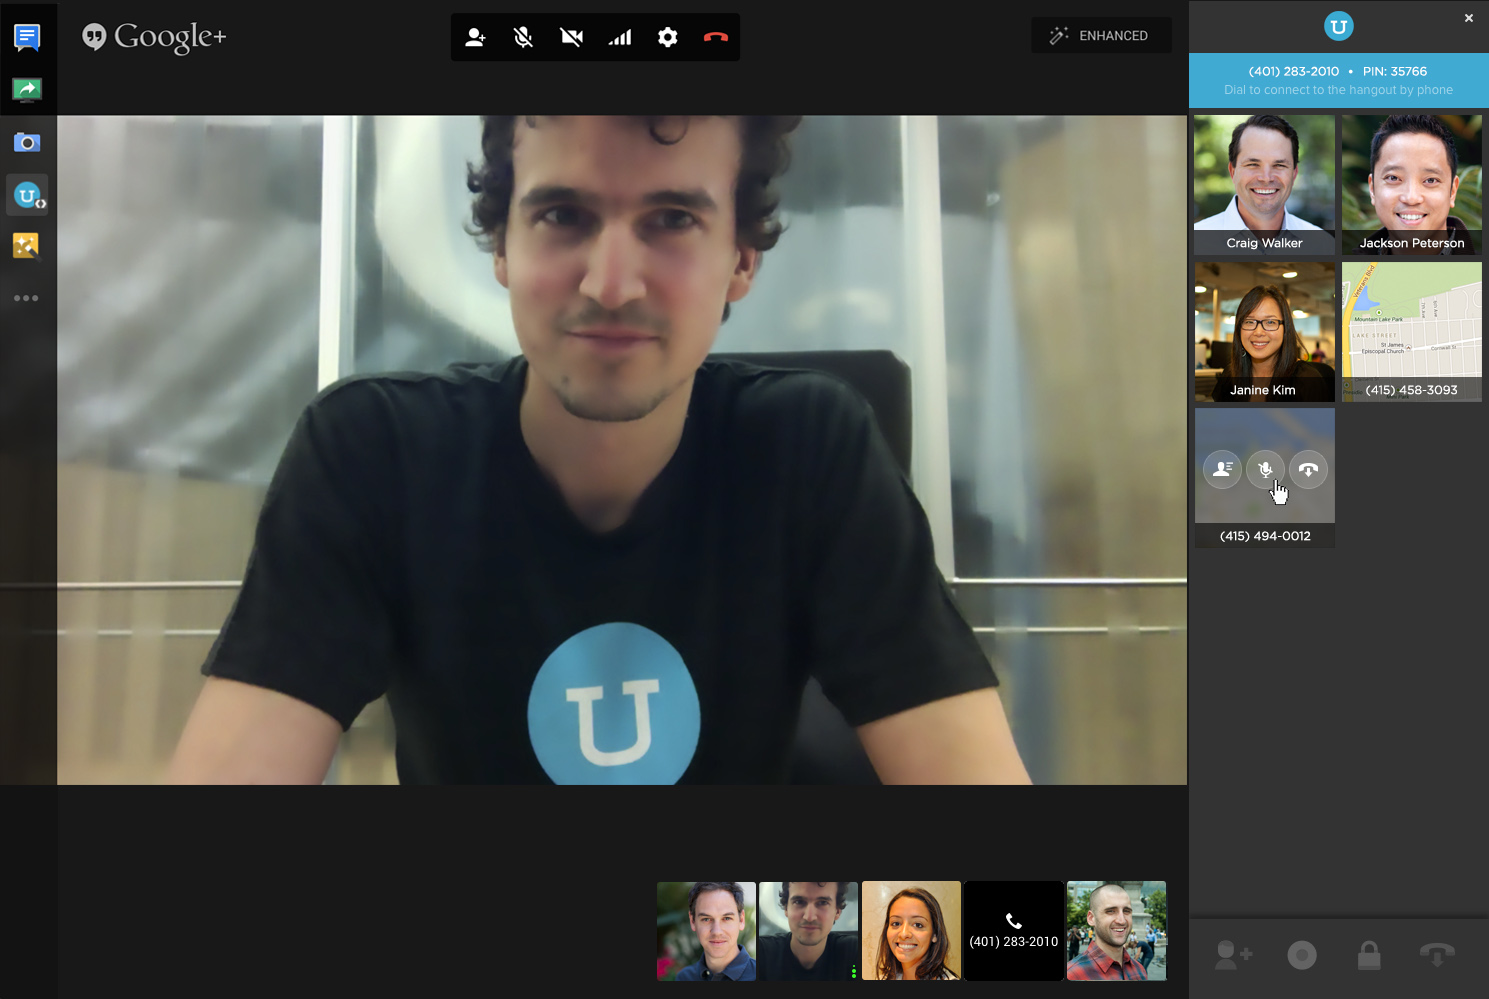
\includegraphics[width=0.58\textwidth,natwidth=610,natheight=642]{figs/uberconference_hangout.jpg}
  	\caption{UberConference integrate with Hangouts Screen shot\cite{tnw:uberconference}}
  	\label{fig:uberconference}
\end{wrapfigure}

\par The prototype system in this thesis is ideally to provide same rich media communication platform as the service provided by UberConference. In February of 2014, UberConference release the new feature which allow user to call into a Google Hangouts session with their mobile phone. The feature is shown in Figure \ref{fig:uberconference}, Once you have installed the UberConference app in Hangouts, people can join your call via phone with the help of a dedicated number. The prototype system will provide the same real-time communication service, but allow the user to create a video conference based on \gls{webrtc} on browser by their mobile phone number and communicate with audio only mobile phone user as well. It will be more easier for user since they just need to remember their user credential related to their mobile phone number in order to use the prototype application rather than register another service user binding with private telephone number. During the real-time conversation, the prototype application will provide user cooperation tools like instance message and file sharing in this development phase.

\subsection{Cube Slam}

\noindent However, there is another important \gls{api}, \textit{RTCDataChannel} , can be used more creatively by the developer to build web applications. The experiment  usage cases, 'Cube Slam' and 'Webtorrent', are in this category which is using \textit{RTCDataChannel} to build \gls{p2p} data sharing without data going though the server to dispatch to other peers. It works more efficiently to handle the synchronization problem.

\par Cube Slam (shown in Figure \ref{fig:cube_slam}) is a Chrome Experiment built with \gls{webrtc} , play an old-school arcade game with your friends without downloading and installing any plug-ins. Cube Slam uses \textit{getUserMedia} to access user's webcam and microphone ,\textit{RTCPeerConnection} to stream user video to another user, and \textit{RTCDataChannel} to transfer the bits that keep the gameplay in sync. If two users are behind firewalls, \textit{RTCPeerConnection} uses a TURN  relay server (hosted on Google Compute Engine) to make the connection. However, when there are no firewalls in the way, the entire game happens directly peer-to-peer, reducing latency for players and server costs for developers.\cite{chrome:cube_slam}

\begin{figure}
	\centering
    	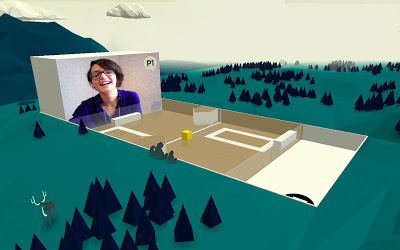
\includegraphics[width=0.8\textwidth,natwidth=610,natheight=642]{figs/cube_slam.jpg}
  	\caption{Cube Slam Game Over Screen}
  	\label{fig:cube_slam}
\end{figure}

\par The idea behind the Cube Slam is that use \textit{RTCDataChannel} to sync the player data in real-time to reduce the latency by peer to peer. \textit{RTCDataChannel} sends data securely, and supports an "unreliable" mode for cases where you want high performance but don't care about every single packet making it across the network. In cases like games where low delay often matters more than perfect delivery, this ensures that a single stray packet doesn't slow down the whole app. The prototype application in this thesis will still use WebSocket for data sharing instead of \textit{RTCDataChannel} because the media server using in this system is not support \textit{RTCDataChannel} yet, so it is not possible to create peer to peer session regarding to this issue. This case about using \textit{RTCDataChannel} in prototype application will be discussed in Chapter \ref{chp:future_work}.

\subsection{Webtorrent}

\par The goal of project Webtorrent is to build a browser BitTorrent client that requires no install, no plugin, no extension, and fully-interoperates with the regular BitTorrent network. It uses \gls{webrtc} Data Channels for peer-to-peer transport. Since WebTorrent is web-first, it's simple for users who do not understand .torrent files, magnet links, NATs, etc. By making BitTorrent easier, it will be accessible to new swathes of users who were previously intimidated, confused, or unwilling to install a program on their machine to participate.\cite{github:webtorrent}

\par Since \gls{webrtc} is usually used for peer to peer communication, the \textit{RTCDataChannel} can be used in more creative way like Webtorrent. Although it need to keep the browser up and running on both ends, then there will be no asynchronous nature into it, it does reduce the bandwidth required and it adds privacy as to who has access to the file being shared. Since the application can reach direct between browsers, it can use the data channel to create a low latency network, where data is shared directly without going through servers on the way. It is lower cost for the developer and more secure on this case. For example, doing the same using a drastically larger number of web browser nodes as \gls{tor}\footnote{Tor (previously an acronym for The Onion Router) is free software for enabling online anonymity and censorship resistance. Tor directs Internet traffic through a free, worldwide, volunteer network consisting of more than five thousand relays to conceal a user's location or usage from anyone conducting network surveillance or traffic analysis.\cite{wiki:tor}}, increases the chance of privacy.This can reduce the need for “real” web servers to run services, and use those only as points of access into the dynamic network that is created ad-hoc.

\section{WebRTC APIs Implementation}

\noindent \gls{webrtc} components are accessed with JavaScript APIs. Currently in development are the Network Stream \gls{api}, which represents an audio or video data stream, and the PeerConnection \gls{api}, which allows two or more users to communicate browser-to-browser. Also under development is a DataChannel \gls{api} that enables communication of other types of data for real-time gaming, text chat, file transfer, and so forth. Because the media server used in prototype system is not support for DataChannel yet, the DataChannel \gls{api} will not be covered in this section.

\begin{figure}
	\centering
    	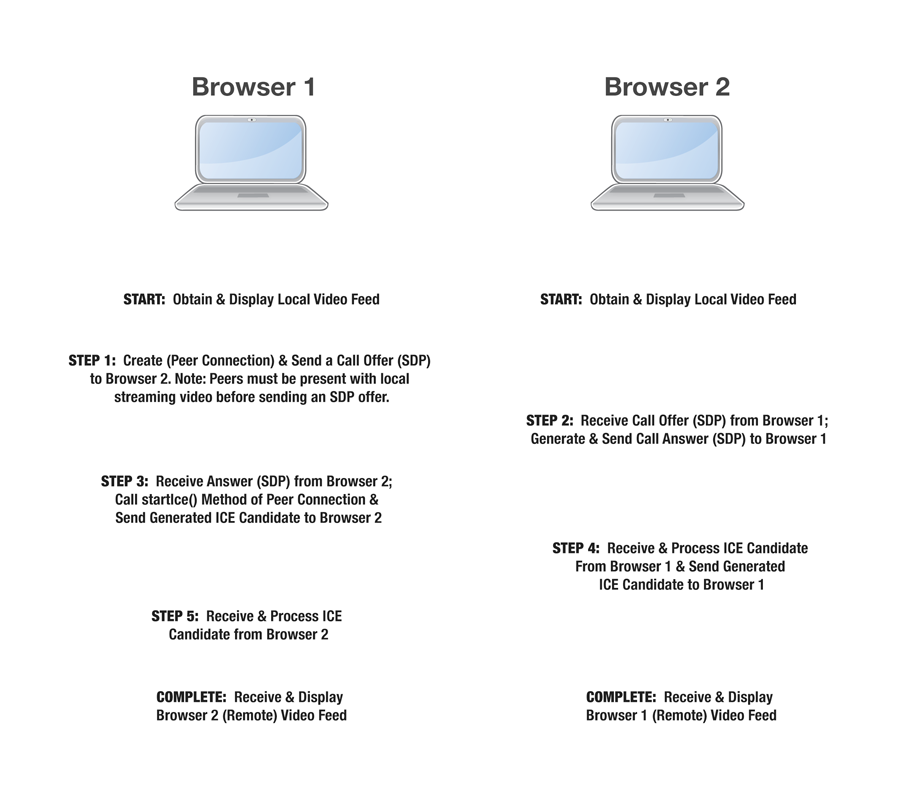
\includegraphics[height=0.50\textheight,natwidth=610,natheight=642]{figs/webrtc_diagram.png}
  	\caption{WebRTC two peer communication process\cite{mdn:p2pwebrtc}}
  	\label{fig:webrtc_diagram}
\end{figure}

\subsection{MediaStream API}

\par The MediaStream \gls{api} represents synchronized streams of media. For example, a stream taken from camera and microphone input has synchronized video and audio tracks. In order to obtain local media, the start step for both peers in Figure \ref{fig:webrtc_diagram} which is a communication process to set up call process from caller peer, the \gls{webrtc} \gls{api}s provide \textit{navigator.getUserMedia()} function to get the video and audio stream from user. For privacy reasons, a web application’s request for access to a user’s microphone or camera will only be granted after the browser has obtained permission from the user. Each MediaStream has an input, which might be a MediaStream generated by \textit{navigator.getUserMedia()}, and an output, which might be passed to a video element or an \textit{RTCPeerConnection}.
\par The \textit{getUserMedia()} method takes three parameters:

\begin{itemize}[topsep=-1em,parsep=0em,itemsep=0em]
 \item A constraints object.
 \item A success callback which, if called, is passed a MediaStream.
 \item A failure callback which, if called, is passed an error object.
\end{itemize}

\par The Code Snippet \ref{code:get_user_media} shows that how the prototype application implements \textit{getUserMedia()} function, it is encapsulated in \textit{WebRTCService} (service is a reusable business logic independent of views in prototype application regarding to AngularJs framework\footnote{AngularJS is an open-source web application framework, maintained by Google and community, that assists with creating single-page applications, one-page web applications that only require HTML, CSS, and JavaScript on the client side.\cite{wiki:angularjs}}). There will be more discuss about prototype application framework in the later part of this chapter. For the constraints object in parameters, the prototype application set 'audio' and 'video' value to true because it is necessary for the real-time communication application to have video and audio stream both.

\begin{lstlisting}[caption={Get User Media Stream function},label={code:get_user_media}]
var media_constraints = {audio: true,video: true};

function _setMediaStream(){
	WebRTCService.getUserMedia(media_constraints,
  								_handleUserMedia,
  								_handleUserMediaError);
  	console.log('Getting user media with constraints', 
  				media_constraints);
}
\end{lstlisting}

\par \textit{getUserMedia()} function is currently available in Chrome, Opera and Firefox. Almost all of the \gls{webrtc} \gls{api}s are slightly different based on different browsers implementation. In the Code Snippet \ref{code:webrtc_service}, from line 40 to line 103 is to make all the set up process for FireFox and from line 106 to line 175 is to make the same set up process for Google Chrome. Because \gls{webrtc} is not standard Web \gls{api} yet, so the implementation on different browsers are different and the \gls{webrtc} \gls{api}s names are slightly different in some browsers. For example, in the Code Snippet \ref{code:webrtc_service} showing, the \textit{RTCPeerConnection} \gls{api} in Firefox is \textit{mozRTCPeerConnection} but in Google Chrome it is \textit{webkitRTCPeerConnection}. In order to make the \gls{webrtc} application works on more browsers, the client side need to figure out which kind of browser is using on the machine then call the corresponding \gls{webrtc} \gls{api}s. Google provides a JavaScript shim called \textit{adapter.js}. It is maintained by Google, it abstracts away browser differences and spec changes. For Angularjs framework used by prototype application, then the \textit{WebRTCService} is implemented to be integrated with \textit{adapter.js} function to achieve the goal of compatibility.

\par However, the prototype application in this thesis will only focus on Google Chrome browser\footnote{Google Chrome is a freeware web browser developed by Google. It used the WebKit layout engine until version 27 and, with the exception of its iOS releases, from version 28 and beyond uses the WebKit fork Blink.\cite{wiki:google_chrome}} to simplify the development process because \gls{webrtc} lower level implementation on different browser s are different and hard to track the issues. Then most of the results in this thesis is based on the application performance of Google Chrome browser. The reason to choose Google Chrome browser rather than other browser because \gls{webrtc} is the technology rapidly pushed by Google and Google Chrome browser has the most market share in the world. As of March 2014, StatCounter estimates that Google Chrome has a 43\% worldwide usage share of web browsers, making it the most widely used web browser in the world.\cite{wiki:google_chrome} However, Google changes a lot to improve the performance of \gls{webrtc} on Google Chrome browser, then it makes the \gls{webrtc} \gls{api}s work different on different version of Google Chrome browser. In the Code Snippet \ref{code:webrtc_service}, from line 124 to line line 136 is the sample case to distinguish the difference among different version of Google Chrome to handle the \textit{RTCPeerConnection} \gls{ice} server constraint implementation.

\par Since \gls{webrtc} \gls{api}s is not standard \gls{api} yet, the prototype application in this thesis will not pay too much work-load on compatibility for different browsers platform. More detail about this issue will be discussed in the Chapter \ref{chp:future_work}.

\subsection{RTCPeerConnection API}

\noindent To set up peer connection, the \textit{RTCPeerConnection} \gls{api} sets up a connection between two peers. In this context, “peers” means two communication endpoints on the World Wide Web. Instead of requiring communication through a server, the communication is direct between the two entities. In the specific case of \gls{webrtc}, a peer connection is a direct media connection between two web browsers. This is particularly relevant when a multi-way communication such as a conference call is set up among three or more browsers. Each pair of browsers will require a single peer connection to join them, allowing for audio and video media to flow directly between the two peers. 

\par To establish peer connection, it requires a new \textit{RTCPeerConnection} object. The only input to the \textit{RTCPeerConnection} constructor method is a configuration object containing the information that \gls{ice}, will use to “punch holes” through intervening \gls{nat} devices and firewalls. The Code Snippet \ref{code:create_peer_connection} shows the create \textit{RTCPeerConnection} object and set three listener (\textit{onicecandidate},\textit{onaddstream},\textit{onremovestream}) to trigger the handlers to deal with the \gls{ice} candidate event and remote stream add/remove events.

\par The \textit{RTCPeerConnection} \gls{api} has two arguments to set, one is configuration object for peer connection and the other is constraint object (set transparent protocol and encryption) for peer connection, these value are shown in Code Snippet \ref{code:create_peer_connection} line 1 to line 10. In the showing case, the prototype is using \gls{stun} servers for different browser aspect, and set the \gls{rtc} channel encryption protocol to \gls{dtls}\footnote{In information technology, the Datagram Transport Layer Security (DTLS) protocol provides communications privacy for datagram protocols. DTLS allows datagram-based applications to communicate in a way that is designed to prevent eavesdropping, tampering, or message forgery.\cite{wiki:dtls}} and enable the \gls{rtc} DataChannel.

\par Because in Firefox, \gls{webrtc} media transparent channel is only based on \gls{dtls} protocol, and in latest version Google Chrome, it is support, then in the prototype application, it will use \gls{dtls} protocol to exchange the media stream.

\par There are two \gls{api}s to handle the \textit{IceCandidate} object which contains \gls{ice} information data. One is \textit{onicecandidate} listener to trigger the function to handle the new \textit{IceCandidate} data object. The other one is \textit{addIceCandidate} function, which is shown in the Code Snippet \ref{code:add_remote_ice}, to add the new \textit{IceCandidate} data object to the remote/local peer connection session description field. 

\begin{lstlisting}[caption={Create Peer Connection function},label={code:create_peer_connection}]
pc_config = WebRTCService.webrtcDetectedBrowser() === 'firefox' ?
  			{'iceServers':[{'urls':'stun:stun.services.mozilla.com'}]} :
  			{'iceServers':[{'urls': 'stun:stun.l.google.com:19302'}]};

pc_constraints = {
			  'optional': [
			    {'DtlsSrtpKeyAgreement': true},
			    {'RtpDataChannels': true}
			  ]
			};
			
function _createPeerConnection(){

	try {
		pc = WebRTCService.peerConnection(pc_config, pc_constraints);
		pc.onicecandidate = _handleIceCandidate;
		console.log('Created RTCPeerConnnection with:\n' +
		      '  config: \'' + JSON.stringify(pc_config) + '\';\n' +
		      '  constraints: \'' + JSON.stringify(pc_constraints) + '\'.');
	} catch (e) {
		console.log('Failed to create PeerConnection, exception: ' + e.message);
		alert('Cannot create RTCPeerConnection object.');
		return;
	}
	pc.onaddstream = _handleRemoteStreamAdded;
	pc.onremovestream = _handleRemoteStreamRemoved;

}
\end{lstlisting}

\begin{lstlisting}[caption={Add Remote IceCandidate function},label={code:add_remote_ice}]
var candidate = WebRTCService.RTCIceCandidate({
					    	sdpMLineIndex:data.content.label,
					    	sdpMid:data.content.id,
					    candidate:data.content.candidate
				});
pc.addIceCandidate(candidate);

\end{lstlisting}

\par In the step 2 of Figure \ref{fig:webrtc_diagram}, after the caller \textit{RTCPeerConnection} run \textit{createOffer()} function to send offer to callee through signaling channel, the callee need run \textit{createAnswer()} function to ask the \gls{stun}/\gls{turn} server to find the path for each other peer and create the answer with \gls{sdp} content. \gls{sdp} is intended for describing multimedia communication sessions for the purposes of session announcement, session invitation, and parameter negotiation. \gls{sdp} does not deliver media itself but is used for negotiation between end points of media type, format, and all associated properties.\cite{wiki:sdp} Before \textit{RTCPeerConnection} use \textit{createOffer()} function to send a \gls{webrtc} offer to the callee, it is required to be present with local streaming video, like Figure \ref{fig:webrtc_diagram} mentioned.

\par The sample \gls{sdp} from the prototype application is shown in Code Snippet \ref{log:webrtc_answer_sdp}. Line 2 in Code Snippet \ref{log:webrtc_answer_sdp} is the field 'o', it describes originator, session identifier, username, id, version number and network address. It usually means that where this package comes from. Line 7 and line 17 are field 'm', it describes media name and transport address. And line 11,12 and line 27,28 are the relevant lines for audio and video media field, they describes media filed 'candidate' attributes, in the sample case of Code Snippet \ref{log:webrtc_answer_sdp}, they are the \gls{ice} candidate from the \gls{stun}/\gls{turn} server. These are important fields regarding to the prototype system because they are used in XMS server and application server of the prototype system.

\begin{lstlisting}[caption={Sample \gls{webrtc} Answer \gls{sdp}},label={log:webrtc_answer_sdp}]
sdp: v=0
o=xmserver 1399363527 1399363528 IN IP4 10.254.9.135
s=xmserver
c=IN IP4 10.254.9.135
t=0 0
a=ice-lite
m=audio 49152 RTP/SAVPF 0 126
a=rtpmap:0 PCMU/8000
a=sendrecv
a=rtcp:49153
a=candidate:1 1 UDP 2130706431 10.254.9.135 49152 typ host
a=candidate:1 2 UDP 2130706430 10.254.9.135 49153 typ host
...
a=acfg:1 t=1
a=rtpmap:126 telephone-event/8000
a=fmtp:126 0-15
m=video 57344 RTP/SAVPF 100
b=AS:1000
a=rtpmap:100 VP8/90000
a=fmtp:100 max-fr=30; max-fs=1200
a=sendrecv
a=rtcp:57345
a=rtcp-fb:100 ccm fir
a=rtcp-fb:100 nack
a=rtcp-fb:100 nack pli
a=rtcp-fb:100 goog-remb
a=candidate:2 1 UDP 2130706431 10.254.9.135 57344 typ host
a=candidate:2 2 UDP 2130706430 10.254.9.135 57345 typ host
...
\end{lstlisting}

\par In the step 3 of Figure \ref{fig:webrtc_diagram}, the caller will receive the answer from callee and process it by adding the remote \gls{sdp} to \textit{RTCPeerConnection}, like the Code Snippet \ref{code:add_remote_ice}. By the meantime, the step 4 of Figure \ref{fig:webrtc_diagram}, the callee will receive the \gls{sdp} from caller with the \gls{ice} candidate information data, and process it the same way as caller does, add some to \textit{RTCPeerConnection} object by \textit{addIceCandidate()} function.

\par \gls{webrtc} clients (known as peers) also need to ascertain and exchange local and remote audio and video media information, such as resolution and codec capabilities. Signaling to exchange media configuration information proceeds by exchanging an offer and an answer using the \gls{sdp}. The \textit{createOffer()} function and \textit{createAnswer()} function both have callback function to handle the \gls{sdp} either to call \textit{setLocalDescription()} by caller or call \textit{setRemoteDescription()} by callee when callee gets the caller's \gls{sdp} from \gls{webrtc} offer. The Code Snippet\ref{log:webrtc_answer_sdp} shown is the \gls{webrtc} answer \gls{sdp} from the callee when the callee end-point decide to accept this conversion session.

\par Once the \textit{RTCPeerConnection} is established, the client need configure where the media or data to store and display if it is necessary. In the prototype application of this thesis, media stream will be displayed in a \gls{html5} tag called \textit{<video>}. It will only be shown when there is media stream in \textit{<video>} tag source.

\section{Prototype Implementation Framework}

\noindent Since \gls{webrtc} is a web \gls{api}, the prototype application will be a web application. There are many different web application framework nowadays to provide rich-client web application. In this section, some of the web application framework will be discussed to figure out which framework is best solution to the prototype scenario. Furthermore, application server is important in the prototype scenario since it does  signaling and bridge the \gls{sip} network and clients.

\subsection{Client Implementation Framework}

\noindent To choose web application framework to implement the client application in this thesis scenario, the main fact is that if the web  application framework is fit to the real time communication application and if the framework has the ability to integrate with \gls{webrtc} \gls{api}. After research about these kind of web application framework, it narrows down to three main framework to discuss.

\textbf{AngularDart :}

\par

\textbf{Sipml5 :}

\par

\textbf{AngularJs + Socket.io: }

\par